% !TeX root = RJwrapper.tex
\title{Navigating the R Package Universe}
\author{by Julia Silge, John C. Nash, Spencer Graves}

\maketitle

\abstract{%
Today, the enormous number of contributed packages available to R users
outstrips any given user's ability to understand how these packages
work, their relative merits, or how they are related to each other. We
organized a plenary session at useR!2017 in Brussels for the R community
to think through these issues and ways forward. This session considered
three key points of discussion. Users can navigate the universe of R
packages with (1) capabilities for directly searching for R packages,
(2) guidance for which packages to use, e.g., from CRAN Task Views and
other sources, and (3) access to common interfaces for alternative
approaches to essentially the same problem.\\
}


\hypertarget{introduction}{%
\subsection{Introduction}\label{introduction}}

As of our writing, there are more than 12,000 packages on CRAN. R users
must approach this abundance of packages with effective strategies to
find what they need and choose which packages to invest time in learning
how to use. At useR!2017 in Brussels, we organized a plenary session on
this issue, with three themes: \textbf{search}, \textbf{guidance}, and
\textbf{unification}. Here, we summarize these important themes, the
discussion in our community both at useR!2017 and in the intervening
months, and where we can go from here.

Users need options to search R packages, perhaps the content of
DESCRIPTION files, documentation files, or other components of R
packages. One author (Graves) has worked on the issue of searching for R
functions from within R itself in the \CRANpkg{sos} package \citep{sos},
and other options have been built such as RDocumentation.org
\citep{rdocumentation}.

Guidance about what package to use for any given task is available from
multiple resources for users. R users can turn to long-established
resources like CRAN Task Views \citep{ctvs}, or newer options under
current development such as \pkg{packagemetrics} \citep{packagemetrics}
or the \CRANpkg{CRANsearcher} RStudio addin \citep{cransearcher}. One
author (Silge) organized a survey before useR about how R users learn
about R packages that informed our discussion and is summarized here.

By unification, we largely mean meta-packages or wrappers, packages that
call other, related packages for a common set of tasks. With a unified
wrapper package, a user only has to learn one API but then can use many
different implementations for a certain task. One author (Nash) has been
particularly involved in numerical optimization techniques and presented
possibilities there and beyond. More generally, as revealed during
breakout discussions at useR!2017 and beyond, there are opportunities to
merge either packages or their functionality. Such ideas require human
cooperation and some give and take in a realm where egos can take
precedence over ease of use.

After our main presentation at useR!2017, we broke out into three
smaller sessions focused on these three themes. We are encouraged by the
engaged attendance and vigorous participation from the community we
experienced, and hope to use our community's enthusiasm and ideas to
move forward with steps that will improve the value of the R ecosystem
to humanity.

\hypertarget{search}{%
\subsection{Search}\label{search}}

There are a number of different search capabilities for R, with
different characteristics and strengths. The ways to search for help
using R have proliferated in much the same way that the number of
packages has, with some of the same challenges. It is not clear to users
what the best way to search is, and many if not most users are not even
aware of the search capabilities that have been built.

The R Project for Statistical Computing's website has had a site focused
on ``Getting Help with R'' \citep{gettinghelp} from early in R's
history. This official overview of various help facilities recognized by
the R Core Team includes functions such as \code{help()}, \code{demo()},
\code{apropos()}, \code{help.search()}, and vignettes. This search and
help functionality, used from R itself, accesses only locally installed
documentation. This site also currently points to resources such as the
CRAN Task Views, FAQ pages, Stack Overflow, and R email lists.

Other search capabilities have been developed by the R community over
the years, focused on different types of searching. The site built by
\citet{baron} is one of the longest running, and can also be accessed
from R itself using the \texttt{RSiteSearch()} function in
\CRANpkg{utils} \citep{utils} and the \CRANpkg{sos} package. The site of
\citet{goodman} is another resource that has been available for over a
decade, and searches not only documentation but also GitHub issues,
social media, and more. The site of \citet{rdrrio} is a newer option
that includes not only a way to search R documentation but also the
ability to run R in the browser. Another full-featured and modern
website for search is RDocumentation.org, which offers users the ability
to contribute examples.

Other options for search capability focus not on documentation or
individual functions but on packages and package descriptions. The
search capability at METACRAN \citep{metacran} and the RStudio addin
\CRANpkg{CRANsearcher} allow users to search the descriptions and titles
of packages to find tools that fit their analysis needs.

This discussion of search options for R users is intended to be thorough
but not entirely exhaustive, and to demonstrate the variety of resources
available. An additional point to be considered is to what extent these
options for search are open source, and what affect that could have,
either positive or negative. For example, the source code for both
METACRAN \citep{metacran} and \CRANpkg{CRANsearcher} is entirely open on
GitHub while RDocumentation.org is maintained by DataCamp, a privately
held company. The analysis in this section is summarized in a
Wikiversity article \citep{wikiversity} and you are invited to
contribute to it.

\hypertarget{guidance}{%
\subsection{Guidance}\label{guidance}}

In preparation for this session, one author (Silge) ran a brief online
survey in the spring of 2017 to ask R users how they currently discover
and learn about R packages. The results of this survey are available in
an R package \pkg{packagesurvey} \citep{packagesurvey} on GitHub. There
were 1039 respondents to this survey, which had a single multiple select
question on it, ``How do you currently discover and learn about R
packages?''

\begin{Schunk}
\begin{table}

\caption{\label{tab:unnamed-chunk-2}Percentage of respondents who chose each answer on survey}
\centering
\begin{tabular}[t]{ll}
\toprule
How do you currently discover and learn about R packages? & \% of respondents\\
\midrule
Social media such as blogs, R-bloggers, Twitter, Slack, or GitHub contacts & 79.8\%\\
General search websites such as Google and Yahoo & 57.0\%\\
Your personal network, such as colleagues and professors & 41.6\%\\
Books, textbooks, or journal articles (JSS, JOSS, R-Journal) & 31.9\%\\
Conferences, meet-ups, or seminars & 24.1\%\\
\addlinespace
CRAN Task Views & 21.8\%\\
Email lists such as r-help, r-packages, or r-pkg-devel & 15.3\%\\
R-specific search websites such as METACRAN or Rdocumentation & 11.1\%\\
Other & 4.2\%\\
R packages built for search such as the sos package & 2.2\%\\
\bottomrule
\end{tabular}
\end{table}

\end{Schunk}

Responses to this survey were fielded from R email help lists, local R
meetup groups, social media such as Twitter, and affinity groups such as
R-Ladies. Figure 1 shows when users responded to the survey. The
respondents to this survey overwhelmingly look to social media including
blogs and Twitter to learn about R packages, and also make use of
general search sites and their personal network.

There were helpful, insightful answers from people contributing to the
``other'' option. R users use
\href{https://stackoverflow.com/questions/tagged/r}{Stack Overflow} to
learn about R packages, as well as options like
\href{http://dirk.eddelbuettel.com/cranberries/}{CRANberries} and
\href{http://www.crantastic.org/}{crantastic}, both of which have RSS
feeds that users follow. Other users mentioned learning by reading code
on GitHub, and other search websites including
\href{http://rpackages.io/}{rpackages.io}.

\begin{Schunk}
\begin{figure}
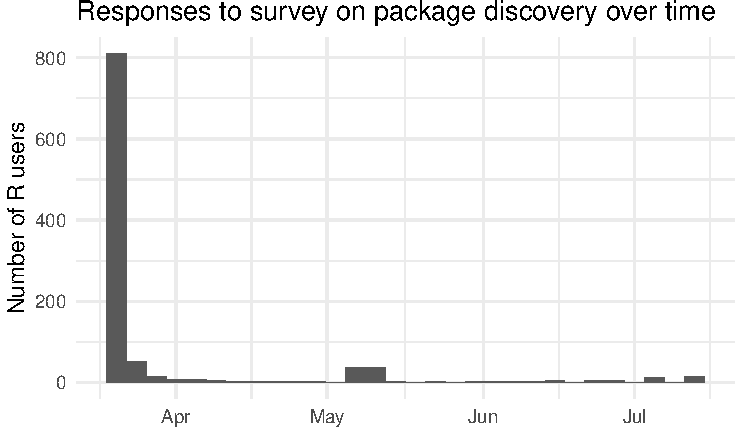
\includegraphics{navigating_files/figure-latex/survey_time-1} \caption[Responses to survey on package discovery during the spring of 2017]{Responses to survey on package discovery during the spring of 2017}\label{fig:survey_time}
\end{figure}
\end{Schunk}

At useR!2017, after the large contributed session, we broke out into
three smaller sessions for discussion and brainstorming. In the breakout
session focused on guidance for package choice and package evaluation,
we had about 40 participants in our discussion. It was a fruitful
discussion and several important themes emerged.

\hypertarget{value-of-personal-impact}{%
\subsubsection{Value of personal
impact}\label{value-of-personal-impact}}

Participants in this session emphasized how impactful personal
relationships can be in how packages are shared and evaluated. Some
participants discussed how building local networks of R users may be
more important in this effort than top-down, technological solutions.
Our survey does show that personal recommendations have been important
for many individuals in evaluating R packages. This is yet another area
where local user groups can continue to have important impact. Some ways
to share this experience more broadly would be online video series or
live data analysis, such as those by
\href{https://www.facebook.com/seanjtaylor/videos/10103088186201897/?pnref=story}{Sean
Taylor} and
\href{https://twitter.com/rdpeng/status/872090694390861824}{Roger Peng}.

\hypertarget{cran-task-views}{%
\subsubsection{CRAN Task Views}\label{cran-task-views}}

Some participants wondered whether the idea of a CRAN Task View
\citep{ctvs} is outdated in the current climate with so many packages,
and whether it is even possible for one person to maintain one
effectively. Others responded that CTVs are focused on curation, which
\emph{is} still important, perhaps even more so now. We had at least one
CTV maintainer present in our breakout session, and several things were
presented as important in order for CTV maintainers to do their jobs:

\begin{itemize}
\tightlist
\item
  Package maintainers should update their \texttt{NEWS} files.
\item
  Package maintainers need to write good documentation.
\end{itemize}

These are helpful for \emph{all} R users, of course, but also for
maintainers of CRAN Task Views. The \CRANpkg{pkgdown} \citep{pkgdown}
package was mentioned as an effective option to make documentation
visible.

\hypertarget{cran-and-you}{%
\subsubsection{\texorpdfstring{CRAN and
\emph{you}}{CRAN and you}}\label{cran-and-you}}

Participants had several ideas about how things are done on CRAN now and
adjustments that might be made in the interest of discovering and
evaluating packages. One idea that came up several times was the
possibility of keywords or tagging for packages. Since useR!2017, the
authors have learned that there is support for some tagging architecture
for packages on CRAN in the
\href{https://cran.r-project.org/doc/manuals/r-release/R-exts.html\#The-DESCRIPTION-file}{DESCRIPTION
file using ACM, JEL, or MSC classifications}. For an example of this in
action, check out the \CRANpkg{lfe} \citep{lfe} package. These are
fairly unwieldy lists currently and something like an RStudio addin
could be used to navigate them, if they were widely used.

Another desire participants voiced was for more information directly on
CRAN, such as the number of downloads for packages. Participants also
suggested that vignettes for context-specific tasks like the
\href{https://www.bioconductor.org/help/workflows/}{Bioconductor
Workflows} would be helpful for package discovery and evaluation, either
associated with CRAN or perhaps the \emph{R Journal}. Finally, there was
some discussion about whether the very minimal gate-keeping on CRAN was
good or bad for the community, although the conclusion was that
editorial efforts to keep packages off CRAN would not be positive.

\hypertarget{more-data-more-problems}{%
\subsubsection{More data, more problems}\label{more-data-more-problems}}

Some of the package developers at the session wondered why, when R is a
data-centric language, developers have such primitive analytics about
their users. Issues of user privacy are central here, but there might be
opt-in options that could help both package developers and users make
better decisions. The idea of a recommender system for R packages was
brought up multiple times, perhaps a Tinder for R packages like
\href{https://simplystatistics.org/2016/10/03/papr/}{papr, the Tinder
for academic preprints}. Both the users and developers present thought
that data on package use (instead of package downloads alone) would be
helpful in evaluating how important or helpful R packages are.
Participants also discussed the possibility of a linter for analysis
scripts, similar in concept to linters for code (such as \citet{lintr}),
that would suggest packages and good practice. Such a linter would
necessarily be opinionated, but almost all efforts to suggest and
evaluate R packages are, by definition.

\hypertarget{unification}{%
\subsection{Unification}\label{unification}}

\textbf{Unification}, as we have describe it here, attempts to reduce
the package count and the span of knowledge required of users. When
there are many ways to carry out the same calculation, there are
inevitable differences of approach. However, in many respects it is the
\textbf{similarity} of approaches that causes most confusion. Very
similar calling sequences, unless they are entirely compatible, lead to
nasty experiences for users, and threaten the validity of results.

From the experience of one author (JN), the most satisfactory form of
unification from the point of view of users is the use of wrapper
functions that consolidate a number of similar tools into a single
calling sequence. This has been the goal of the package
\CRANpkg{optimx}, which in its 2018 incarnation consolidates a number of
R-internal and package-based function minimization tools. Moreover, the
present version subsumes a number of other packages, thereby offering a
reduction in the effective package count.

The downside of this is the amount of work for the developer. Worse, the
very large package count has led to many \textbf{reverse dependencies}.
At the time of writing, the new \CRANpkg{optimx} fails checks of reverse
dependencies, though apparently not because of anything new in the
package. The issues seem to relate to general tightening-up of checks
for CRAN policies, so that the dependent packages fail (or are not
installable) \textbf{before} they even try functionality from
\CRANpkg{optimx}. Such issues will have to be resolved.

While a wrapper such as \CRANpkg{optimx} can, with effort, be created,
merging two existing but different packages that provide similar
capability with very different user interfaces requires human
cooperation. At this time, and despite the very collaborative R
community, the level of effort to do such work is daunting. Moreover,
there is a general lack of financial or other reward for such efforts.

During discussions at useR!2017, it was clear that R users are quite
interested in unification of packages. Younger participants expressed
the opinion that there were egos and interest groups standing in the way
of some such unifications, and the status of some of the players impeded
the discussion of such possibilities.

\hypertarget{summary}{%
\subsection{Summary}\label{summary}}

Our work on these topics leads us to call for increased respect and
value for the work done by local meetup group organizers and individuals
who contribute to spreading R knowledge, both online and in their
communities. Our survey and discussions show how impactful these
community networks are; investing in community building is not something
we need do only because of idealism, but because it is effective.

We can also see the importance of continued commitment to growing the
skills of package developers across the R ecosystem. Adopting best
practices, including understanding dependency management and writing
good documentation, makes this entire challenge better for everyone,
from the developer with downstream dependencies to the CRAN Task View
maintainer to the new R user.

JOHN AND SPENCER: For full details of \emph{The R Journal} style and
information on how to prepare your article for submission, see the
\href{https://journal.r-project.org/share/author-guide.pdf}{Instructions
for Authors}.

\bibliography{RJreferences}


\address{%
Julia Silge\\
Stack Overflow\\
110 William Street, Floor 28\\ New York City, NY 10038\\
}
\href{mailto:julia.silge@gmail.com}{\nolinkurl{julia.silge@gmail.com}}

\address{%
John C. Nash\\
University of Ottawa\\
Telfer School of Management\\ Ottawa, ON K1N 6N5, Canada\\
}
\href{mailto:nashjc@uottawa.ca}{\nolinkurl{nashjc@uottawa.ca}}

\address{%
Spencer Graves\\
EffectiveDefense.org\\
4550 Warwick Blvd. Apt. 508\\ Kansas City, MO 64111\\
}
\href{mailto:spencer.graves@effectivedefense.org}{\nolinkurl{spencer.graves@effectivedefense.org}}

